%!TEX root = 00_main.tex

\section{Rendering Photo-Realistic Images}

\begin{figure}
	\captionsetup[subfigure]{labelformat=empty} % stop subcaption writing "(a)""
    \captionsetup{subrefformat=parens} % add parentheses to \subref
    \centering
    \begin{subfigure}[t]{0.48\columnwidth}
        \inlinelabel{a}{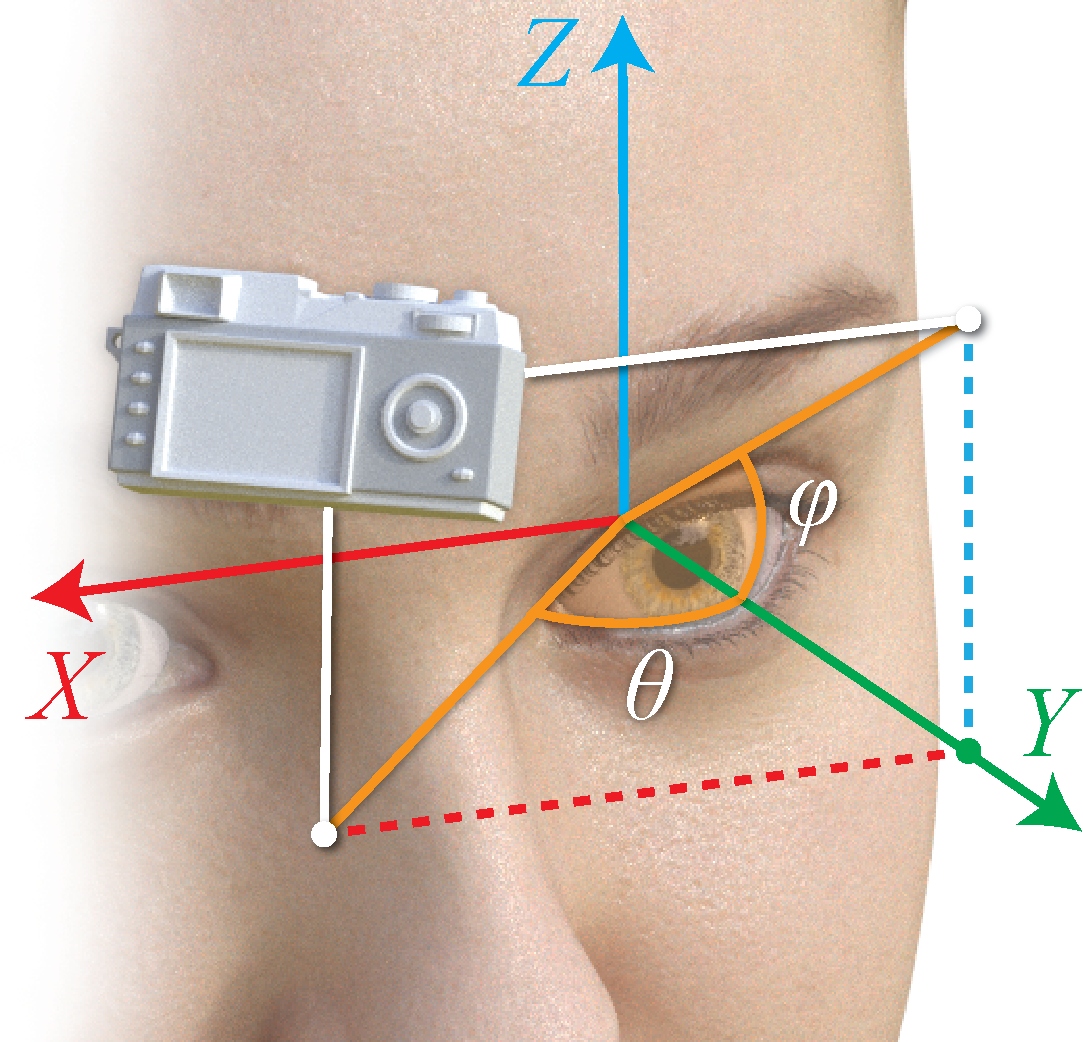
\includegraphics[width=\textwidth]{camera_position}}
        \caption{}\label{fig:cam_pos_spher_coords}
    \end{subfigure}
    \hfill
    \begin{subfigure}[t]{0.48\columnwidth}
        \inlinelabel{b}{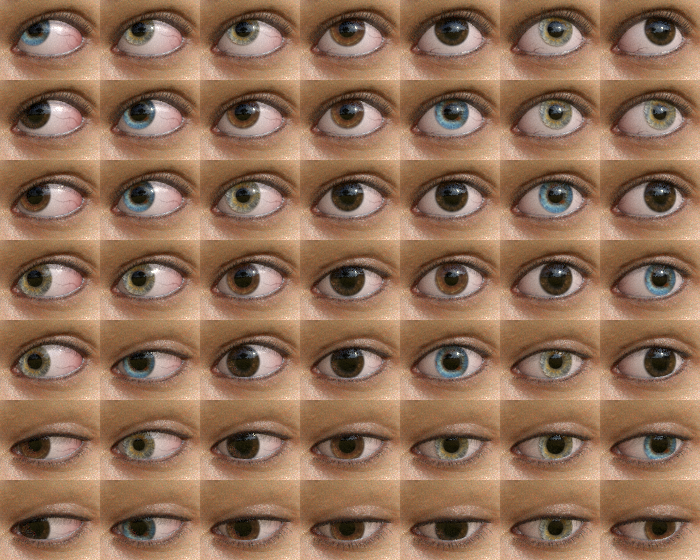
\includegraphics[width=\textwidth]{camera_pos_sample_renders_7x7}}
        \caption{}\label{fig:cam_pos_example_renders}
    \end{subfigure}
    \par\vspace{-28pt}
    \caption{The camera is positioned to simulate changes in head pose \subref{fig:cam_pos_spher_coords}. At each position, we render many eye images for different gaze directions by posing the eyeball model \subref{fig:cam_pos_example_renders}.}
    \label{fig:cam_pos}
\end{figure}

% reword?
In-the-wild images exhibit huge amounts of appearance variability across different viewpoints and illumination. Our goal was to sufficiently sample our model across these degrees of variation to create a representitive dataset.
In this section we first describe how we pose our viewpoint and model, then we explain how we use image-based lighting~\cite{debevec2002image} to model a wide range of realistic environments, and finally discuss the details of our rendering setup.

\subsection{Posing the model}

% not sure if its worthwhile trying to formally parameterize the rendering model in the paper
% might be simpler to just use words?
For a chosen eye-region model configuration, each rendered image is determined by parameters $(\mathbf{c}, \mathbf{g}, L)$: 3D camera position $\mathbf{c}$; 3D gaze vector $\mathbf{g}$; and lighting environment $L$.
As shown in \autoref{fig:cam_pos}, camera positions $\mathbf{c}$ were chosen by iterating over spherical coordinates $(r, \theta, \phi)$, centered around the eyeball center.
We used orthographic rendering, as this simulates an eye region-of-interest being cropped from a wide-angle camera image, so we set $r\!=\!1$ for convenience.
At each camera position $\mathbf{c}$, we rendered multiple images with different 3D gaze vectors to simulate the eye looking in different directions.
Examples with fixed $L$ are shown in \autoref{fig:cam_pos_example_renders}.
Gaze vectors $\mathbf{g}$ were chosen by first pointing the eye directly at the camera (simulating eye-contact), and then modifying the eyeball's pitch ($\alpha$) and yaw ($\beta$) angles over a chosen range.
For our generic \dataset dataset, we rendered images with up to $45^{\circ}$ horizontal and vertical deviation from eye-contact, in increments of $10^{\circ}$.
%
As we posed the model in this way, there was the possibility of rendering ``unhelpful'' images that either simulate impossible scenarios or are not useful for training.
To avoid violating anatomical constraints, we only rendered images for valid eyeball rotations $|\alpha|\!\leq\!25^{\circ}$ and $|\beta|\!\leq\!35^{\circ}$ \cite{MIL-STD-1472G}.
Before rendering, we also verified that the projected 2D pupil center in the image was within the 2D boundary of the eyelid landmarks -- this prevented us from rendering images where too little of the iris was visible.

\subsection{Creating realistic illumination}

\begin{figure}
    \begin{subfigure}[t]{\columnwidth}
        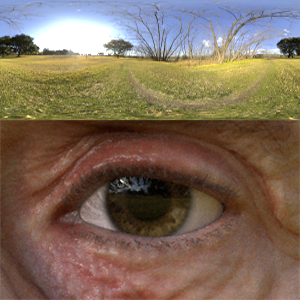
\includegraphics[width=0.24\textwidth]{fig_env_1} \hfill
    	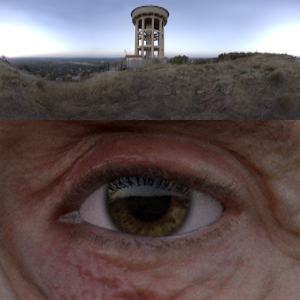
\includegraphics[width=0.24\textwidth]{fig_env_2} \hfill
        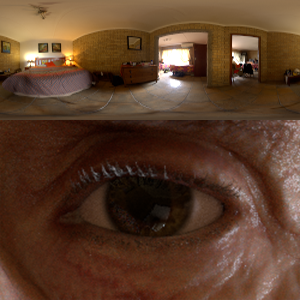
\includegraphics[width=0.24\textwidth]{fig_env_3} \hfill
    	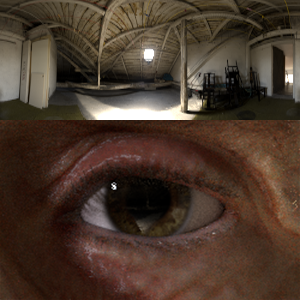
\includegraphics[width=0.24\textwidth]{fig_env_4}
	    \caption{The four HDR environment maps we use for realistic lighting: bright/cloudy outdoors, and bright/dark indoors}
    \end{subfigure}
    \par \medskip
    \begin{subfigure}[t]{0.48\columnwidth}
        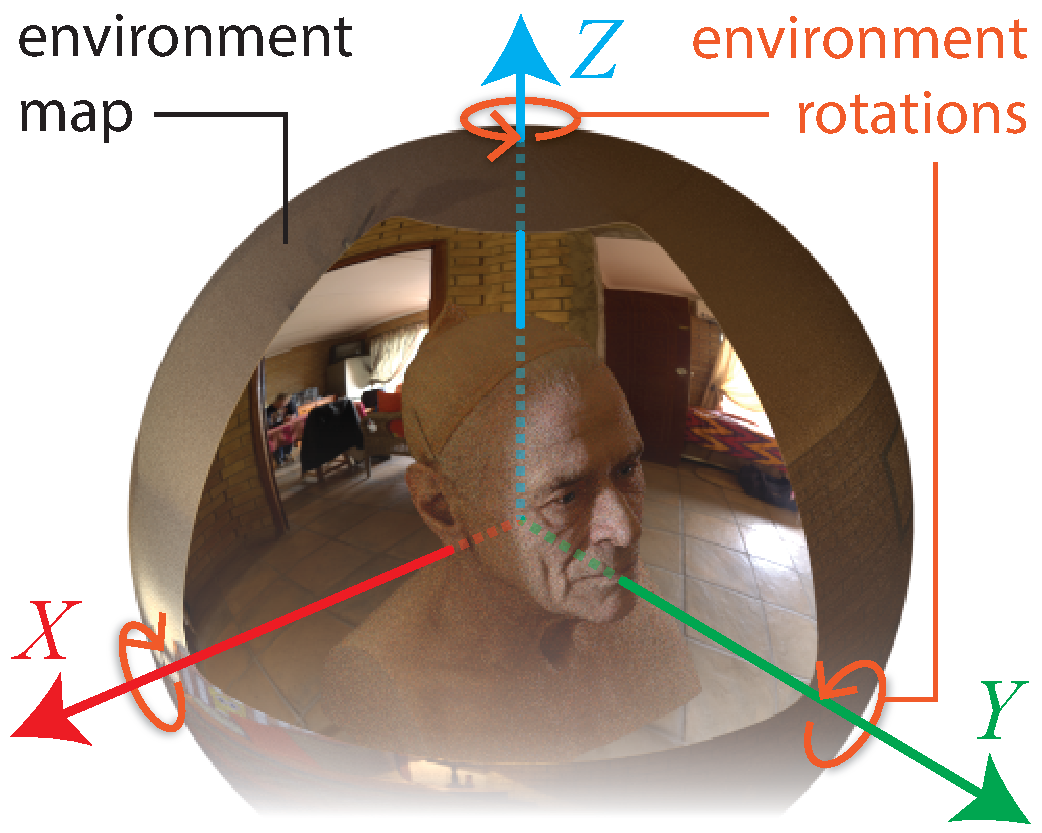
\includegraphics[width=\textwidth]{env_explain_5x4}
    	\caption{The environment is rotated to simulate different head poses}
    \end{subfigure}%
    \hfill
    \begin{subfigure}[t]{0.48\columnwidth}
        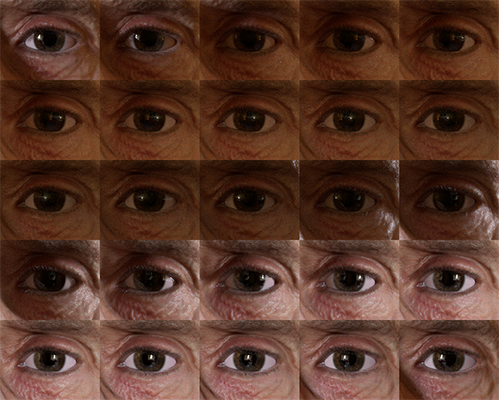
\includegraphics[width=\textwidth]{env_variation}
        \caption{Renders using a single environment, rotated about $Z$}
        \label{fig:env_map_imgs_examples}
    \end{subfigure}
    \caption{Appearance variation from lighting is modelled with poseable high dynamic range environment maps \cite{debevec2002image}.}
    \label{fig:environment_maps}
\end{figure}

One of the main challenges in computer vision is illumination invariance -- a good system should work under a range of real-life lighting conditions.
We realistically illuminate our eye-model using \emph{image-based lighting}, a technique where high dynamic range (HDR) panoramic images are used to provide light in a scene \cite{debevec2002image}.
This works by photographically capturing omni-directional light information, storing it in a texture, and then projecting it onto a sphere around the object.
When a ray hits that texture during rendering, it takes that texture's pixel value as light intensity.
At render time we randomly chose one of four freely available HDR environment images to simulate a range of different lighting conditions (see \autoref{fig:environment_maps}) \cite{AdaptiveSamplesHDR}.
The environment is then randomly rotated to simulate a continuous range of head-pose, and randomly scaled in intensity to simulate changes in ambient light.
As shown in \autoref{fig:env_map_imgs_examples}, a combination of hard shadows and soft light can generate a range of appearances from only a single HDR environment.
This simple and flexible approach creates varaibility using measured light levels in representitive environments rather than randomly configuring light sources and ambient lights \cite{zface}.

\subsection{Rendering engine}

We use Blender's inbuilt Cycles path-tracing engine for rendering \cite{Cycles}.
This Monte Carlo method traces the paths of many light rays per pixel, scattering light stochastically off physically-based materials in the scene until they reach illuminants.
A GPU implementation is available for processing large numbers of rays simultaneously ($150/\textrm{px}$) to achieve noise-free and photorealistic images.
Each $120\!\times\!80\textrm{px}$ eye-region image rendering took $5.26\textrm{s}$ on average across all head models using a commodity GPU (Nvidia GTX660).
Our generic head-pose and gaze-direction dataset of 11,000 images can be rendered in under a day on a single machine, though in practice we rendered using multiple machines simultaneously.
As a result we can quickly generate a large, representitive, high-quality dataset with clean labels in a fraction of the time taken by traditional data collection procedures \cite{zhang15_cvpr} \todo{cite more}.